\documentclass[letter]{article}
\renewcommand{\baselinestretch}{1.25}

\usepackage[margin=1in]{geometry}
\usepackage{physics}
\usepackage{amsmath}
\usepackage{graphicx}
\usepackage{hyperref}


% MATLAB Formating Code
\usepackage[numbered,framed]{matlab-prettifier}
\lstset{style=Matlab-editor,columns=fullflexible}
\renewcommand{\lstlistingname}{Script}
\newcommand{\scriptname}{\lstlistingname}

\allowdisplaybreaks

%opening
\title{MECH 6313 - Homework 1}
\author{Jonas Wagner}
\date{2021, February 1}

\begin{document}

\maketitle


\section{Problem 1 - Hopf Bifurcation}
\subsection{Part a}
\textbf{Problem:}
Simulate the following system for various parameters to determine the type of bifurcation that occurs:
\begin{equation}
	\begin{aligned}
		\dot{x} &= \alpha x + y\\
		\dot{y} &= -x + \alpha y - x^2 y
	\end{aligned}
\end{equation}

\noindent
\textbf{Solution:}
The system was simulated for various parameter values and initial conditions using MATLAB's built-in ode45 solver. The MATLAB code for this assignment is available in \appendixname \ref{script:HW1}\\

\begin{figure}[h]
	\centering
	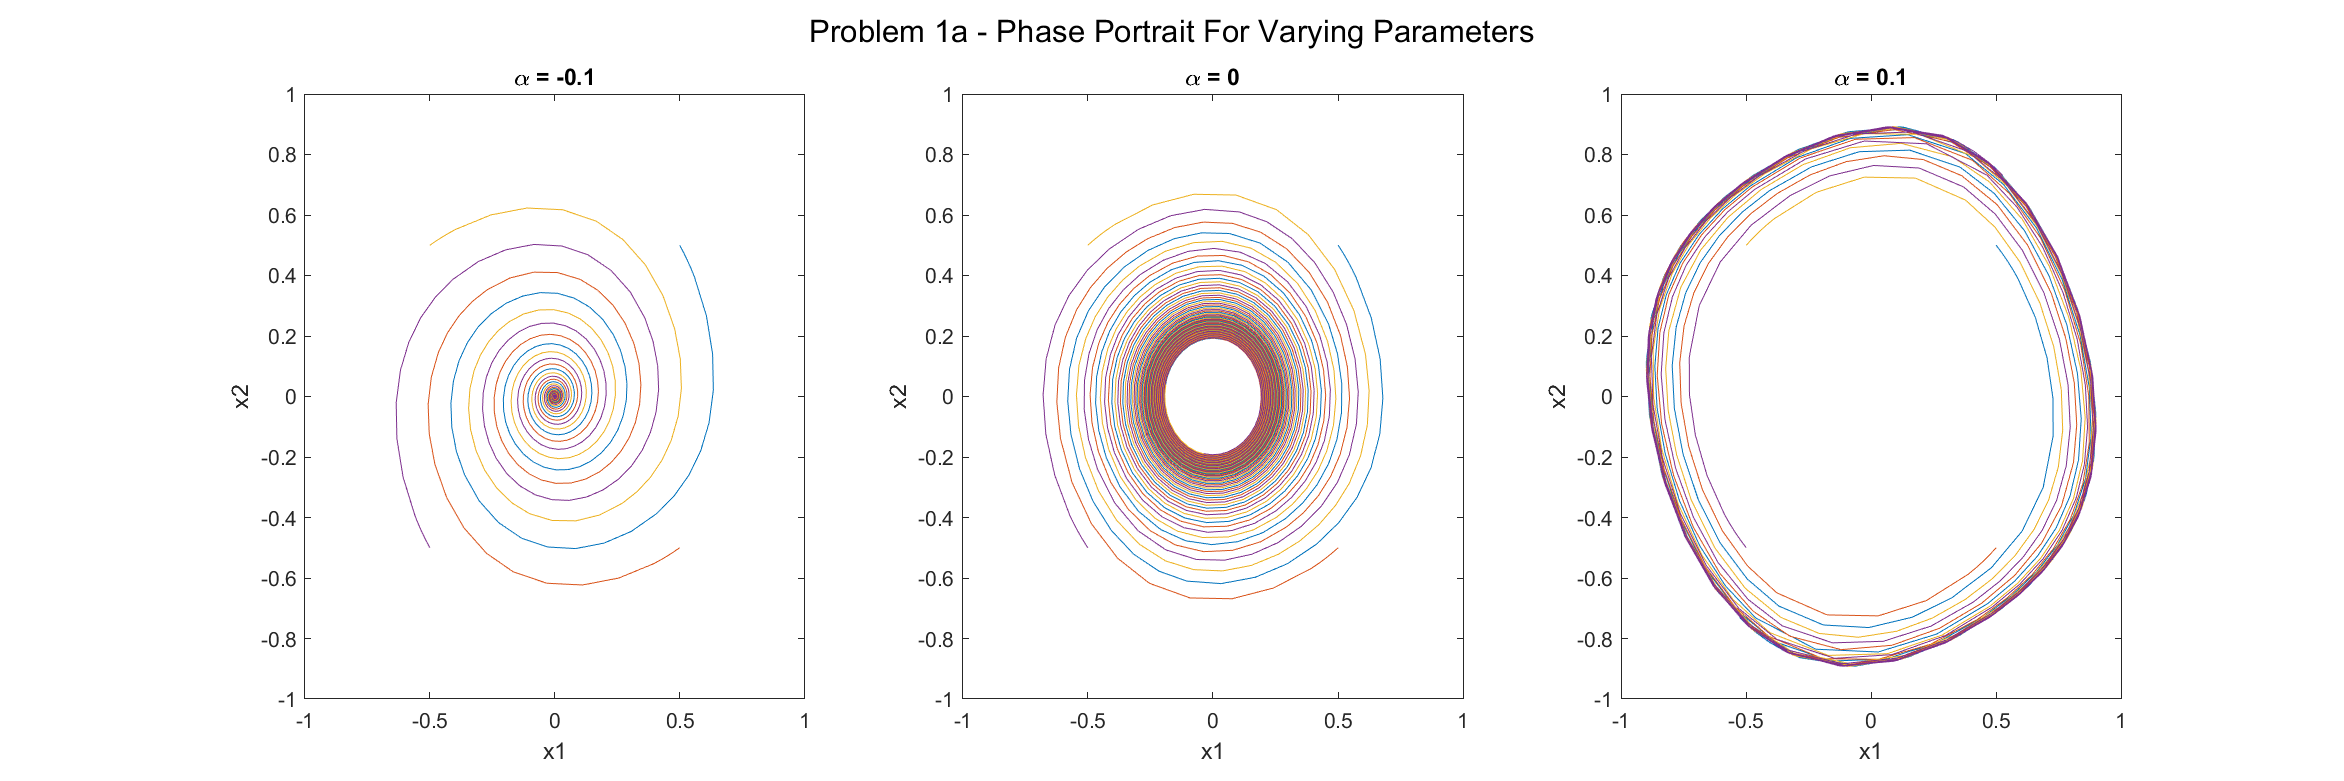
\includegraphics[width=1\linewidth]{fig/pblm1a}
	\caption{Phase Plot of the system for various values of $\alpha$ and initial conditions}
	\label{fig:pblm1a}
\end{figure}

The numerical solution clearly shows a stable limit cycle for $\alpha > 0$, thus it exhibits supercritical hopf bifucation.



\newpage
\subsection{Part b}
\textbf{Problem:}
Simulate the following system for various parameters to determine the type of bifurcation that occurs:
\begin{equation}
	\begin{aligned}
		\dot{x} &= \alpha x + y - x^3\\
		\dot{y} &= -x + \alpha y + 2 y^3
	\end{aligned}
\end{equation}

\noindent
\textbf{Solution:}
The system was simulated for various parameter values and initial conditions using MATLAB's built-in ode45 solver. The MATLAB code for this assignment is available in \appendixname \ref{script:HW1}\\

\begin{figure}[h]
	\centering
	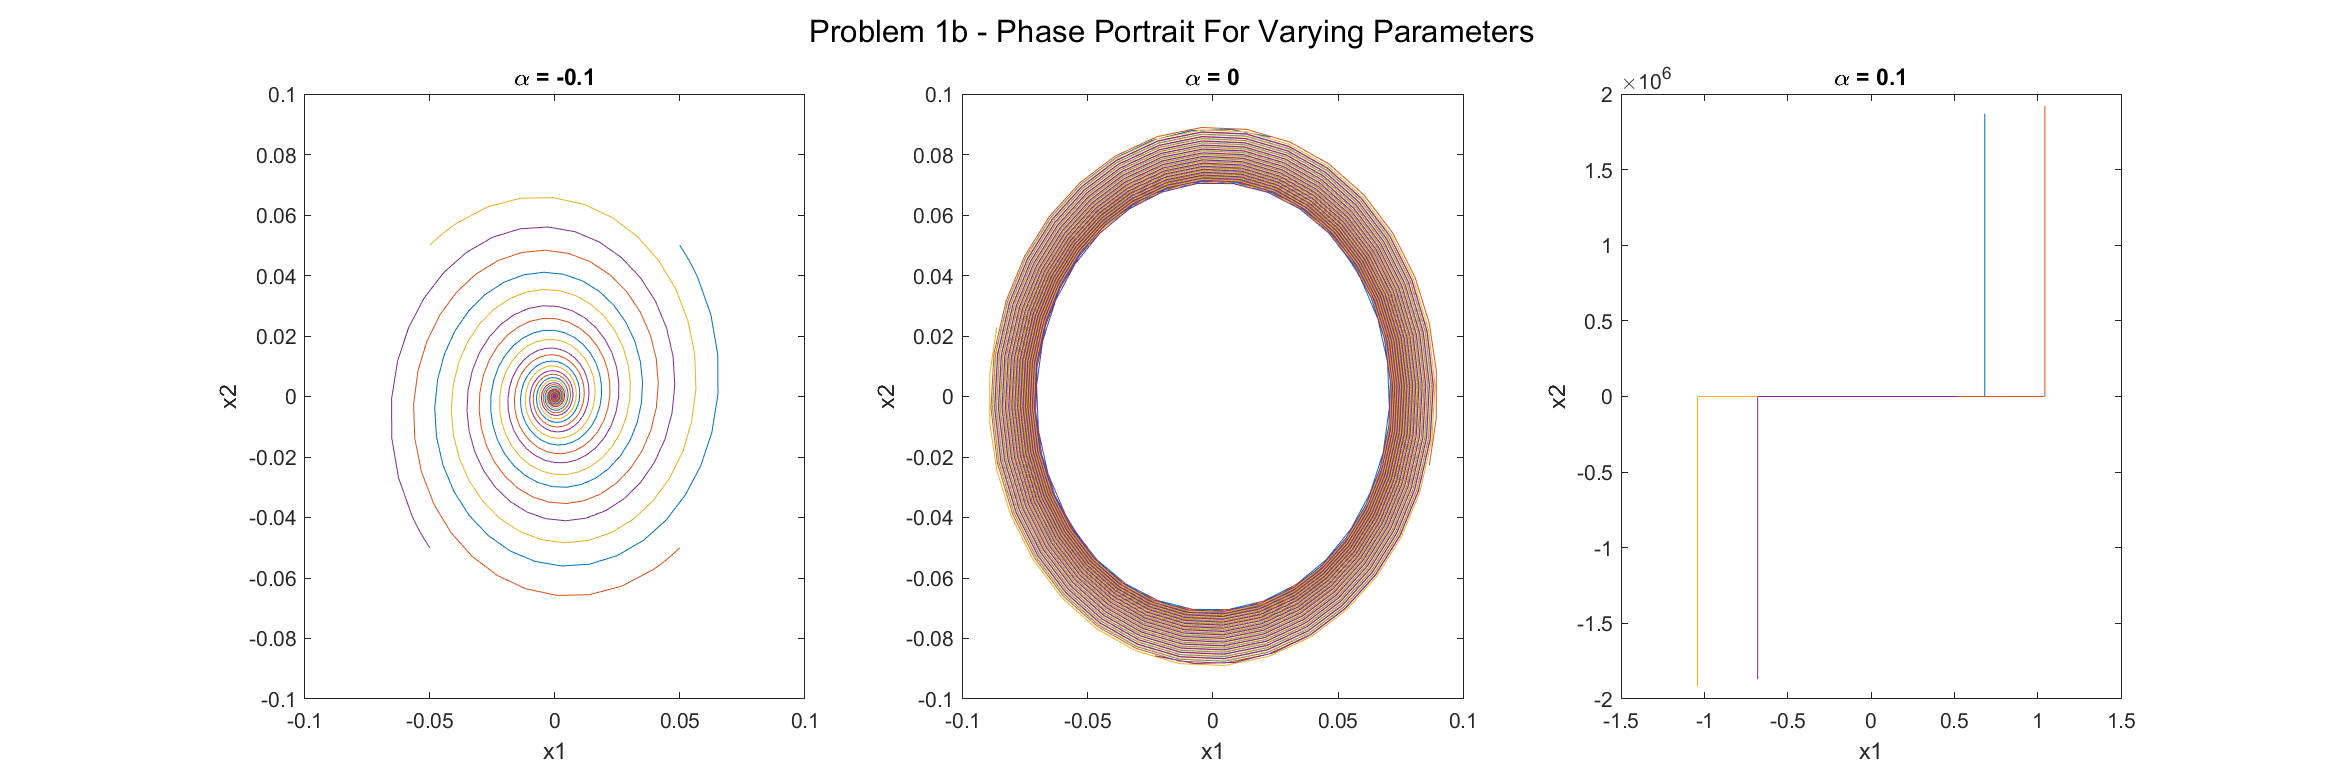
\includegraphics[width=1\linewidth]{fig/pblm1b}
	\caption{Phase Plot of the system for various values of $\alpha$ and initial conditions}
	\label{fig:pblm1b}
\end{figure}

The numerical solution clearly shows a very unstable system for $\alpha > 0$, thus it exhibits subcritical hopf bifucation. One interesting occurrence though is the limit cycle that is occurring for $\alpha \approx 0$.

\newpage
\subsection{Part c}
\textbf{Problem:}
Simulate the following system for various parameters to determine the type of bifurcation that occurs:
\begin{equation}
	\begin{aligned}
		\dot{x} &= \alpha x + y - x^2\\
		\dot{y} &= -x + \alpha y + 2 x^3
	\end{aligned}
\end{equation}

\noindent
\textbf{Solution:}
The system was simulated for various parameter values and initial conditions using MATLAB's built-in ode45 solver. The MATLAB code for this assignment is available in \appendixname \ref{script:HW1}\\

\begin{figure}[h]
	\centering
	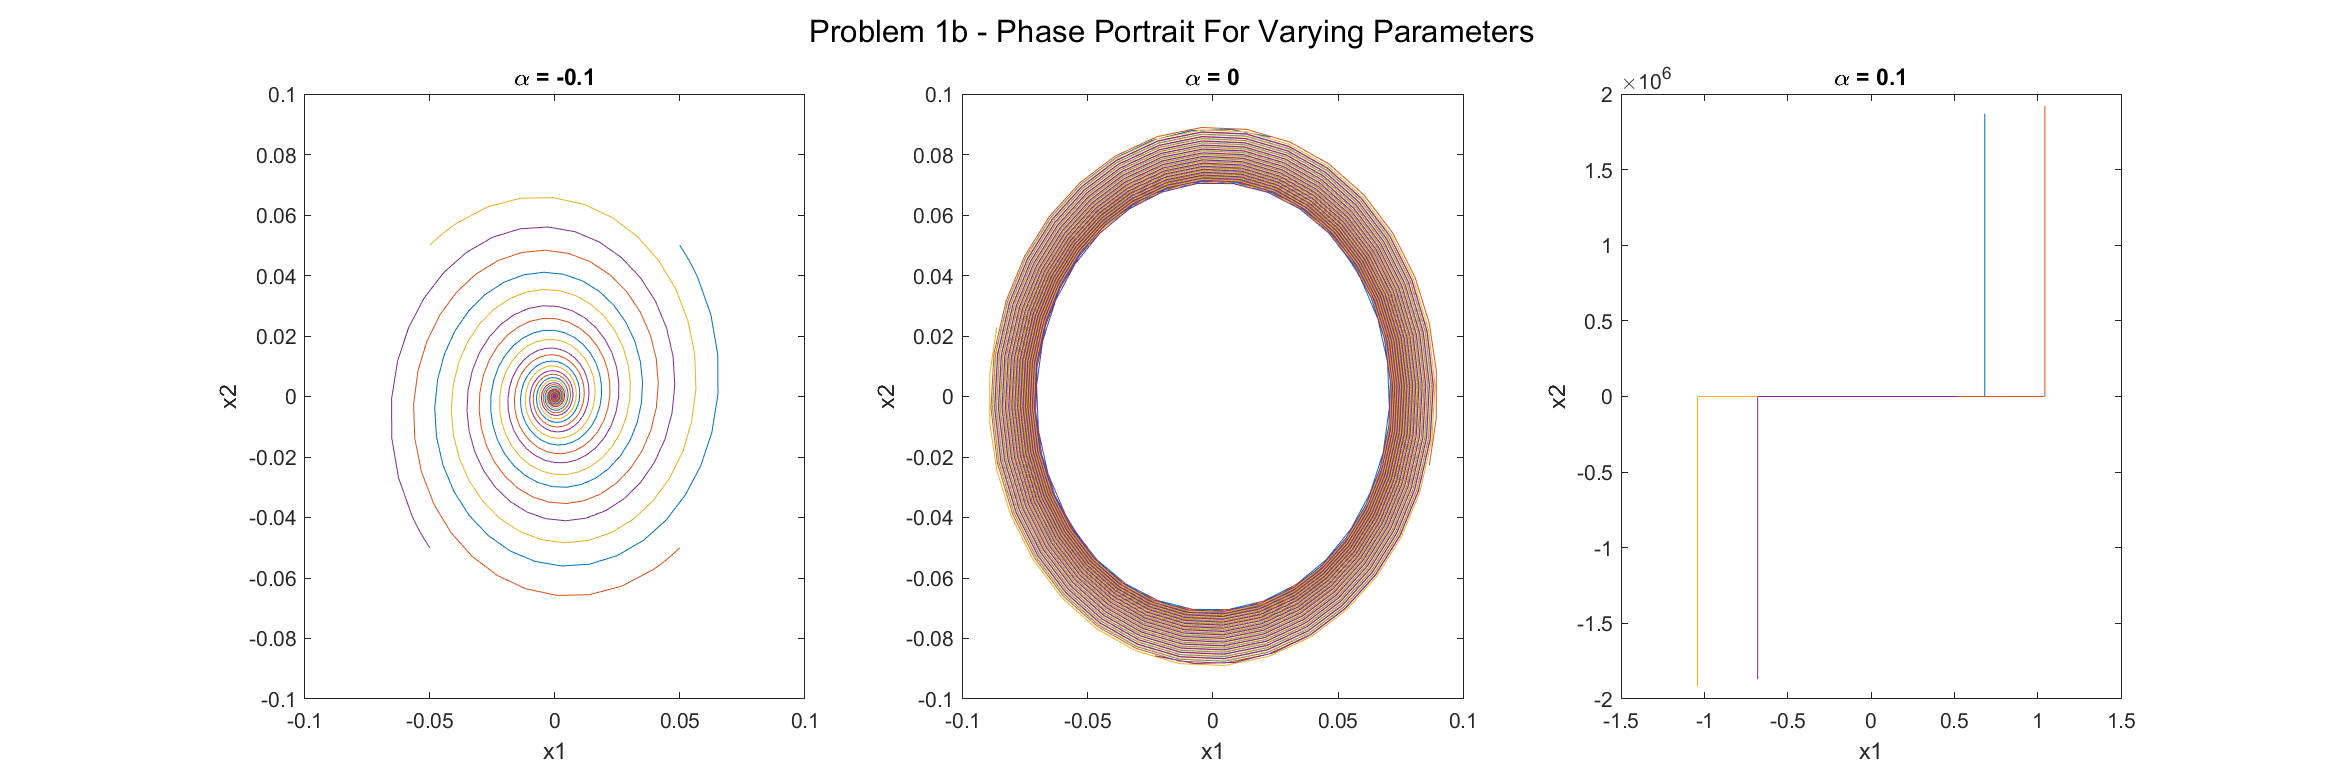
\includegraphics[width=1\linewidth]{fig/pblm1b}
	\caption{Phase Plot of the system for various values of $\alpha$ and initial conditions}
	\label{fig:pblm1c}
\end{figure}

The numerical solution clearly shows unstable behavior for $\alpha > 0$, thus it exhibits subcritical hopf bifucation.


\newpage
\section{Problem 2}

\subsection{Part a}

\subsubsection{System Linearization}
\textbf{Problem:}
Linearize and analyze the following system.
\begin{equation}
	\begin{aligned}
		\dot{x}_1 &= x_2 + x_1 x_2^2\\
		\dot{x}_2 &= -x_1 + x_1^2 x_2
	\end{aligned}
\end{equation}

\noindent
\textbf{Solution:}
The linearized solution can be calculated by determining the first-order taylor expansion of the nonlinear system:
\begin{equation}
	f(x) \approx f(x_0) + \eval{\dv{f}{x}}_{x=x_0} \bar{x} + H.O.T., \ \ \bar{x} = x - x_0
\end{equation}

In this case, the $A$ matrix is calculated as the Jacobian of the system dynamics evaluated at $x=x_0=0$:

\begin{align}
	A = \eval{\dv{f}{x}}_{x=x_0} 
	&= \eval{\mqty[\pdv{f_1}{x_1} & \pdv{f_1}{x_2}\\
				  \pdv{f_2}{x_1} & \pdv{f_2}{x_2}]}_{x=x_0}
  	, \ \ x_0 = \mqty[0\\0]\\
  	&= \eval{\mqty[x_2^2 & 2 x_1 x_2 + 1\\
  					2 x_1 x_2 -1 & x_1^2]}_{x_1 = x_2 = 0}\\
	&= \mqty[0 & 1\\ -1 & 0]
\end{align}

The linear dynamics for the equilibrium point is therefore given as:
\begin{equation}
	\vb{\dot{x}} = A \vb{x} = \mqty[0 & 1\\ -1 & 0] \vb{x}
\end{equation}

The characteristics roots are therefore calculated as the eigenvalues of $A$:
$$\lambda_{1,2} = \pm j$$

From this we can conclude the linear system is a harmonic oscillator that is marginally stable.

\newpage
\subsubsection{Bendixon's Criteria}
\textbf{Problem:}
Show that the system has no closed orbits.\\

\noindent
\textbf{Solution:}
Bendixon's Criterion states that if the divergence of $f(x)$ is not equivalently zero and does not change sign with a simply connected region then there are no periodic orbits in that region.\\

The divergence of the system can be calculated as:
\begin{align}
	\div f  &= \pdv{f_1}{x_1} + \pdv{f_2}{x_2} \nonumber\\
	&= x_1^2 + x_2^2
\end{align}

Let $D$ be defined as the region satisfying $0 < x_1^2 + x_2^2 \leq r^2$, then there does exist an $r>0$ in which Bendixon's Criterion applies. (In this case $r$ can be $\infty$). This is sufficient to say that there are no periodic orbits exist (even though the linear system at the equilibrium point suggests this is the case).


\subsection{Part b}
\subsubsection{Bendixon's Criteria}
\textbf{Problem:}
Show that the following system has no closed orbits:
\begin{equation}
	\begin{aligned}
		\dot{x}_1 &= x_1 x_2^3\\
		\dot{x}_2 &= x_1
	\end{aligned}
\end{equation}

\noindent
\textbf{Solution:}
Bendixon's Criterion states that if the divergence of $f(x)$ is not equivalently zero and does not change sign with a simply connected region then there are no periodic orbits in that region.\\

The divergence of the system can be calculated as:
\begin{align}
	\div f  &= \pdv{f_1}{x_1} + \pdv{f_2}{x_2} \nonumber\\
	&= x_2^3 + 0 \nonumber\\
	&= x_2^3
\end{align}

First, let $D1$ and $D2$ be defined as the entire upper and lower planes respectively:
\begin{equation}
	\begin{aligned}
		D1 &:= \{x \in \real^2 \ | \ x_2 < 0\}\\
		D2 &:= \{x \in \real^2 \ | \ x_2 > 0\}
	\end{aligned}
\end{equation}

Within the regions $D1$ and $D2$, the divergence is strictly negative and positive respectively. Thus for each region the Bendixon Criteria applies and they independently contain no periodic orbits.
Additionally, whenever $x_2 = 0$ an equilibrium point exists. This is sufficent to say that the entire domain contains no periodic orbits.



\newpage
\section{Problem 3}
\textbf{Problem:}
For each of the following systems demonstrate that no limit cycles exist:

\noindent
\textbf{Solution:}
\subsection{2.20.1}
Let the following system be defined
\begin{equation}
	\begin{aligned}
		\dot{x}_1 &= -x_1 + x_2\\
		\dot{x}_2 &= g(x_1) + a x_2
	\end{aligned}
\end{equation}
where $g(x)$ is an arbritrary function and $a \neq 1$.

The divergence of the system can be calculated as:
\begin{align}
	\div f  &= \pdv{f_1}{x_1} + \pdv{f_2}{x_2} \nonumber\\
	&= -1 + a\\
	&= a - 1
\end{align}

Given $a \neq 1$, it is true that the divergence of the system is always a constant not equal to zero. This satisfies Bendixon's Criteron for the entire domain. This is sufficient to prove no periodic orbits exist, and thus no limit cycles can exist.

\newpage
\subsection{2.20.2}
Let the following system be defined
\begin{equation}
	\begin{aligned}
		\dot{x}_1 &= -x_1 + x_1^3 + x_1 x_2^2\\
		\dot{x}_2 &= -x_2 + x_2^3 + x_1^2 x_2
	\end{aligned}
\end{equation}

The divergence of the system can be calculated as:
\begin{align}
	\div f  &= \pdv{f_1}{x_1} + \pdv{f_2}{x_2} \nonumber\\
	&= 3x_1^2 + x_2^2 - 1 + 3 x^2 + x_1^2 - 1\\
	&= 4 x_1^2 + 4 x_2^2 - 2
\end{align}

For the region $$D = \{x\in \real^2 \ | \ 4 x_1^2 + 4 x_2^2 < 2\}$$, the Bendixon Criteron applies as the divergence is always positive. This is also true for the compliment of $D$.

This is not true for the border region,
\begin{equation}
	B = \{x \in \real^2 \ | \ 4 x_1^2 + 4 x_2^2 = 2\}
\end{equation}
however the system is unstable for the entire boarder. This can be seen by analyzing the Jacobian with $x_0 \in B$:

\begin{align}
	\eval{\dv{f}{x}}_{x=x_0} 
	&= \eval{\mqty[\pdv{f_1}{x_1} & \pdv{f_1}{x_2}\\
		\pdv{f_2}{x_1} & \pdv{f_2}{x_2}]}_{x=x_0}\\
	&= \eval{\mqty[3 x_1^2 + x_2^2 -1 & 2 x_1 x_2\\
					2 x_1 x_2 & x_1^2 + 3 x_2^2 -1]}_{x=x_0}
\end{align}
The eigenvalues of the Jacobian matrix can be calculated to be:
\begin{equation}
	\begin{aligned}
		\lambda_1 &= x_1^2 + x_2^2 -1\\
		\lambda_2 &= 3 x_1^2 + 3 x_2^2 - 1
	\end{aligned}
\end{equation}

This can then be evaluated for the boarder region $B$ to be
\begin{equation}
	\lambda_{1,2} = \pm \frac{1}{2}
\end{equation}

Due to the unstable pole at $\frac{1}{2}$ this disqualifies a limit cycle from occurring at the boarder.\\

Given both the conclusion of the Bendixon Criterion and the unstable boundary, it can be said that no limit cycles exist.


\newpage
\subsection{2.20.3}
Let the following system be defined
\begin{equation}
	\begin{aligned}
		\dot{x}_1 &= 1 - x_1 x_2^2\\
		\dot{x}_2 &= x_1
	\end{aligned}
\end{equation}


The divergence of the system can be calculated as:
\begin{align}
	\div f  &= \pdv{f_1}{x_1} + \pdv{f_2}{x_2} \nonumber\\
	&= -x_2 + 0\\
	&= - x_2
\end{align}

For the regions defined as
\begin{equation}
	\begin{aligned}
		D_1 &:= \{x \in \real^2 \ | \ x_2 \leq 0\}\\
		D_2 &:= \{x \in \real^2 \ | \ x_2 \geq 0\}
	\end{aligned}
\end{equation}
divergence remains positive and negative for $D_1$ and $D_2$ respectively.\\

This is not true for the border region,
\begin{equation}
	B = \{x \in \real^2 \ | \ x_2 = 0\}
\end{equation}
however the system is unstable for the entire boarder.

This can be seen by analyzing the Jacobian with $x_0 \in B$:

\begin{align}
	\eval{\dv{f}{x}}_{x=x_0} 
	&= \eval{\mqty[\pdv{f_1}{x_1} & \pdv{f_1}{x_2}\\
		\pdv{f_2}{x_1} & \pdv{f_2}{x_2}]}_{x=x_0}\\
	&= \eval{\mqty[-x_2^2 & -2 x_1 x_2\\ 1 & 0]}_{x=x_0}
\end{align}
The eigenvalues of the Jacobian matrix can be calculated and evaluated for the boarder region $B$.
\begin{equation}
	\lambda_{1,2} = 0
\end{equation}

Due to the unstable pole at $0$ this disqualifies a limit cycle from occurring at the boarder.\\

Given both the conclusion of the Bendixon Criterion and the unstable boundary, it can be said that no limit cycles exist.


\newpage
\subsection{2.20.4}
Let the following system be defined
\begin{equation}
	\begin{aligned}
		\dot{x}_1 &= x_1 x_2\\
		\dot{x}_2 &= x_2
	\end{aligned}
\end{equation}

The divergence of the system can be calculated as:
\begin{align}
	\div f  &= \pdv{f_1}{x_1} + \pdv{f_2}{x_2} \nonumber\\
	&= 1 + x_2
\end{align}

For the region $$D = \{x\in \real^2 \ | \ x_2 > -1\}$$, the Bendixon Criteron applies as the divergence is always positive. This is also true for the compliment of $D$ as the divergence is always negative.

This is not true for the border region,
\begin{equation}
	B = \{x \in \real^2 \ | \ x_2 = -1\}
\end{equation}
however the system is unstable for the entire boarder. This can be seen by analyzing the Jacobian with $x_0 \in B$:

\begin{align}
	\eval{\dv{f}{x}}_{x=x_0} 
	&= \eval{\mqty[\pdv{f_1}{x_1} & \pdv{f_1}{x_2}\\
		\pdv{f_2}{x_1} & \pdv{f_2}{x_2}]}_{x=x_0}\\
	&= \eval{\mqty[x_2 & x_1\\ 0 &1]}_{x=x_0}
\end{align}
The eigenvalues of the Jacobian matrix can be calculated to be:
\begin{equation}
	\begin{aligned}
		\lambda_1 &= 1
		\lambda_2 &= x_2
	\end{aligned}
\end{equation}

This can then be evaluated for the boarder region $B$ to be
\begin{equation}
	\lambda_{1,2} = \pm 1
\end{equation}

Due to the unstable pole at $\lambda = 1$ this disqualifies a limit cycle from occurring at the boarder (plus its a line...).\\

Given both the conclusion of the Bendixon Criterion and the unstable boundary, it can be said that no limit cycles exist.




\newpage
\subsection{2.20.5}
Let the following system be defined
\begin{equation}
	\begin{aligned}
		\dot{x}_1 &= x_2 \cos(x_1)\\
		\dot{x}_2 &= \sin(x_1)
	\end{aligned}
\end{equation}

The divergence of the system can be calculated as:
\begin{align}
	\div f  &= \pdv{f_1}{x_1} + \pdv{f_2}{x_2} \nonumber\\
	&= -x_2 \sin(x_1)
\end{align}

Let the following regions be defined:
\begin{equation}
	\begin{aligned}
		D_1 := \{x \in \real^2 \ | \ n \pi < x_1 < (n \pi +\frac{\pi}{2}) \ \forall n = 0, 1, \dots \text{ and } x_2 < 0\}\\
		D_2 := \{x \in \real^2 \ | \ n \pi < x_1 < (n \pi +\frac{\pi}{2}) \ \forall n = 0, 1, \dots \text{ and } x_2 > 0\}\\
		D_3 := \{x \in \real^2 \ | \ (n \pi +\frac{\pi}{2}) < x_1 < n \pi \ \forall n = 0, 1, \dots \text{ and } x_2 < 0\}\\
		D_4 := \{x \in \real^2 \ | \ (n \pi +\frac{\pi}{2}) < x_1 < n \pi \ \forall n = 0, 1, \dots \text{ and } x_2 > 0\}\\
	\end{aligned}
\end{equation}

Each of the regions individualy satisfy Bendixon's criterion as $D_1$ and $D_4$ are always positive while $D_2$ and $D_3$ are always negative.\\

For the points not included in the the 4 regions,
\begin{equation}
	\begin{aligned}
		B_1 &:= \{x \in \real^2 \ | \ x_1 = n \pi \ \forall n = 0, 1, \dots\}\\
		B_2 &:= \{x \in \real^2 \ | \ x_1 = \frac{\pi}{2} + n \pi \ \forall n = 0, 1, \dots\}
	\end{aligned}
\end{equation}
it can be shown that each is an equilibrium point.

This can be seen by analyzing the Jacobian with $x_0 \in B_1 \text{ and } B_2$:
\begin{align}
	\eval{\dv{f}{x}}_{x=x_0} 
	&= \eval{\mqty[\pdv{f_1}{x_1} & \pdv{f_1}{x_2}\\
		\pdv{f_2}{x_1} & \pdv{f_2}{x_2}]}_{x=x_0}\\
	&= \eval{\mqty[-x_2 sin(x_1) & cos(x_1)\\ cos(x_1) & 0]}_{x=x_0}
\end{align}

The eigenvalues of the Jacobian matrix for $B_1$ can be calculated and evaluated as
\begin{equation}
	\lambda_{1,2} = \pm 1
\end{equation}

Similarily,the eigenvalues of the Jacobian matrix for $B_2$ can be calculated and evaluated as
\begin{equation}
	\lambda_{1,2} = 0
\end{equation}

Given both the conclusion of the Bendixon Criterion and the unstable boundary, it can be said that no limit cycles exist.




\newpage
\section{Problem 4}
A nonlinear system is defined as:
\begin{equation}
	\begin{aligned}
		\dot{x_1} &= x_2\\
		\dot{x_2} &= -[2b - g(x_1)]ax_2 - a^2 x_1
	\end{aligned}
\end{equation}
where $a,b>0$ and
\begin{equation}
	g(x_1) = 
	\begin{cases}
		0 & \abs{x_1} > 1\\
		k & \abs{x_1} \leq 1
	\end{cases}
\end{equation}

\subsection{Bendixson's Criterion}
\textbf{Problem:}
Use Bendixson's Criterion to prove no periodic orbits exists if $k < 2b$.

\noindent
\textbf{Solution:}\\
Fist let the following domains be defined:
\begin{equation}
	\begin{aligned}
		D_1 := \{x \in \real^2 \ | \ \abs{x_1} \leq 1\}\\
		D_2 := \{x \in \real^2 \ | \ \abs{x_1} > 1\}
	\end{aligned}
\end{equation}

The divergence of the system in $D_1$ can be calculated as:
\begin{align}
	\div f  &= \pdv{f_1}{x_1} + \pdv{f_2}{x_2} \nonumber\\
	&= 0 - (2b - 0)a\\
	&= - 2ab
\end{align}
In this case the divergence will also always be negative.\\


Similarly, the divergence of the system in $D2$ can be calculated as:
\begin{align}
	\div f  &= \pdv{f_1}{x_1} + \pdv{f_2}{x_2} \nonumber\\
	&= 0 - (2b - k)a\\
	&= (k - 2b)a
\end{align}
In the case that $k < 2b$, it can be seen that the divergence will always be negative.\\

From this it can be concluded using Bendixson's Criterion that no periodic orbits exist.

\newpage
\subsection{Poincare-Bendixon Criterion}
\textbf{Problem:}
Use Poincare-Bendixon Criteron to show that these is a periodic orbit if $k > 2b$.

\noindent
\textbf{Solution:}
The Jacobian for the region $D_1$ is given as
\begin{align}
	\eval{\dv{f}{x}}_{x=x_0} 
	&= \eval{\mqty[\pdv{f_1}{x_1} & \pdv{f_1}{x_2}\\
		\pdv{f_2}{x_1} & \pdv{f_2}{x_2}]}_{x=x_0}\\
	&= \eval{\mqty[0 & 1\\ -a^2 & -a(2b - k)]}_{x=x_0}
\end{align}


The Jacobian for the region $D_2$ is given as
\begin{align}
	\eval{\dv{f}{x}}_{x=x_0} 
	&= \eval{\mqty[\pdv{f_1}{x_1} & \pdv{f_1}{x_2}\\
		\pdv{f_2}{x_1} & \pdv{f_2}{x_2}]}_{x=x_0}\\
	&= \eval{\mqty[0 & 1\\ -a^2 & -a(2b)]}_{x=x_0}
\end{align}

Looking at a region region around the only equalibrium point:
\begin{align}
	M &:= \{x \in \real^2 \ | \ r^2 \leq x_1^2 + x_2^2 \leq R^2\}
	\intertext{Then the scaler field defined as:}
	V(x) &= x_1^2 + x_2^2\\
	\intertext{The gradient is then defined by}
	\grad{V(x)} &= \mqty[2x_1\\ 2x_2]\\
	\intertext{The normal component of the system dynamics can then be found with:}
	F^T(x) \cdot \grad{V(x)} &= \mqty[x_2 & - a(2b - g(x_1))x_2 - a^2 x_1] \mqty[2x_1\\ 2x_2]\\
	&= 2 x_1 x_2 - 2 a(2b - g(x_1))x_2^2 - 2 a^2 x_1 x_2\\
	\intertext{When the region $M = D_1$ this becomes:}
	F^T(x) \cdot \grad{V(x)} &= 2 x_1 x_2 (1 - a^2) - 4ab x_2^2\\
	\intertext{When the region $M = D_1$ this becomes:}
	F^T(x) \cdot \grad{V(x)} &= 2 x_1 x_2 (1 - a^2) + (2ak - 4ab) x_2^2
	\intertext{Since $x_1 \leq 1$, the following must hold:}
	-4 a b + 2 ak &> 0\\
	2ak &> 4ab\\
	k &> 2b
\end{align}

This means that $M$ is positive invariant for $k > 2b$, therefore from the Poincare-Bendixon Criteron, there must be a periodic orbit.



\newpage
\appendix
\section{MATLAB Code:}
All code I write in this course can be found on my GitHub repository:\\
\href{https://github.com/jonaswagner2826/MECH6313}{https://github.com/jonaswagner2826/MECH6313}
% MECH6313_HW1
\lstinputlisting[caption={MECH6313\_HW1},label={script:HW1}]{MECH6313_HW2.m}


\end{document}
